\chapter{亚伯拉罕 Rachael?,Leo}
\section{亞伯蘭经文}
\subsection{中文}
\subsubsection{應許萬族因亞伯蘭得福 11:31-32/12:1-7}
他拉带着他的儿子亚伯兰和他的孙子，就是哈兰的儿子罗得，以及他的媳妇亚伯兰的妻子撒莱，一同出了迦勒底的吾珥，要到迦南地去；他们到了哈兰，就住在那里。 32他拉死在哈兰；他的寿数共二百零五岁。

耶和華對亞伯蘭說：「你要離開本地、本族、父家，往我所要指示你的地去。 2 我必叫你成為大國，我必賜福給你，叫你的名為大，你也要叫別人得福。 3 為你祝福的，我必賜福於他；那咒詛你的，我必咒詛他。地上的萬族都要因你得福。」 4 亞伯蘭就照著耶和華的吩咐去了，羅得也和他同去。亞伯蘭出哈蘭的時候年七十五歲。 5 亞伯蘭將他妻子撒萊和侄兒羅得，連他們在哈蘭所積蓄的財物、所得的人口，都帶往迦南地去。他們就到了迦南地。6 亞伯蘭經過那地，到了示劍地方，摩利橡樹那裡。那時，迦南人住在那地。 7 耶和華向亞伯蘭顯現，說：「我要把這地賜給你的後裔。」亞伯蘭就在那裡為向他顯現的耶和華築了一座壇。 





\subsubsection{神應許亞伯蘭之後裔多如眾星 15:2-8}
亚伯兰说：“主耶和华啊，我既无子，你还赐我什么呢？并且要承受我家业的是大马士革人以利以谢。” 3 亚伯兰又说：“你没有给我儿子，那生在我家中的人就是我的后嗣。” 4 耶和华又有话对他说：“这人必不成为你的后嗣，你本身所生的才成为你的后嗣。” 5 于是领他走到外边，说：“你向天观看，数算众星，能数得过来吗？”又对他说：“你的后裔将要如此。” 6 亚伯兰信耶和华，耶和华就以此为他的义。 7 耶和华又对他说：“我是耶和华，曾领你出了迦勒底的吾珥，为要将这地赐你为业。” 8 亚伯兰说：“主耶和华啊，我怎能知道必得这地为业呢？” 
\subsubsection{神應許亞伯蘭之後裔多如眾星 15:13-21}
耶和華對亞伯蘭說：「你要的確知道，你的後裔必寄居別人的地，又服侍那地的人，那地的人要苦待他們四百年。 14 並且他們所要服侍的那國，我要懲罰，後來他們必帶著許多財物從那裡出來。 15 但你要享大壽數，平平安安地歸到你列祖那裡，被人埋葬。 16 到了第四代，他們必回到此地，因為亞摩利人的罪孽還沒有滿盈。」 17 日落天黑，不料有冒煙的爐並燒著的火把從那些肉塊中經過。 18 當那日，耶和華與亞伯蘭立約，說：「我已賜給你的後裔，從埃及河直到伯拉大河之地， 19 就是基尼人、基尼洗人、甲摩尼人、 20 赫人、比利洗人、利乏音人、 21 亞摩利人、迦南人、革迦撒人、耶布斯人之地。」




\subsubsection{神易亞伯蘭為亞伯拉罕 17:1-8}
亞伯蘭年九十九歲的時候，耶和華向他顯現，對他說：「我是全能的神，你當在我面前做完全人。 2 我就與你立約，使你的後裔極其繁多。」 3 亞伯蘭俯伏在地，神又對他說： 4 「我與你立約：你要做多國的父。 5 從此以後，你的名不再叫亞伯蘭，要叫亞伯拉罕，因為我已立你做多國的父。 6 我必使你的後裔極其繁多，國度從你而立，君王從你而出。 7 我要與你並你世世代代的後裔堅立我的約，做永遠的約，是要做你和你後裔的神。 8 我要將你現在寄居的地，就是迦南全地，賜給你和你的後裔永遠為業，我也必做他們的神。」



\subsubsection{神試驗亞伯拉罕 22:1-3}
這些事以後，神要試驗亞伯拉罕，就呼叫他說：「亞伯拉罕！」他說：「我在這裡。」 2 神說：「你帶著你的兒子，就是你獨生的兒子，你所愛的以撒，往摩利亞地去，在我所要指示你的山上，把他獻為燔祭。」 3 亞伯拉罕清早起來，備上驢，帶著兩個僕人和他兒子以撒，也劈好了燔祭的柴，就起身往神所指示他的地方去了。 

\subsubsection{神試驗亞伯拉罕 22:4-8}
4 到了第三日，亞伯拉罕舉目遠遠地看見那地方。 5 亞伯拉罕對他的僕人說：「你們和驢在此等候，我與童子往那裡去拜一拜，就回到你們這裡來。」 6 亞伯拉罕把燔祭的柴放在他兒子以撒身上，自己手裡拿著火與刀，於是二人同行。 7 以撒對他父親亞伯拉罕說：「父親哪！」亞伯拉罕說：「我兒，我在這裡。」以撒說：「請看，火與柴都有了，但燔祭的羊羔在哪裡呢？」 8 亞伯拉罕說：「我兒，神必自己預備做燔祭的羊羔。」於是二人同行。


\subsubsection{神試驗亞伯拉罕 22:9-18}
9 他們到了神所指示的地方，亞伯拉罕在那裡築壇，把柴擺好，捆綁他的兒子以撒，放在壇的柴上。 10 亞伯拉罕就伸手拿刀，要殺他的兒子。 11 耶和華的使者從天上呼叫他說：「亞伯拉罕！亞伯拉罕！」他說：「我在這裡。」 12 天使說：「你不可在這童子身上下手，一點不可害他。現在我知道你是敬畏神的了，因為你沒有將你的兒子，就是你獨生的兒子，留下不給我。」 13 亞伯拉罕舉目觀看，不料，有一隻公羊，兩角扣在稠密的小樹中。亞伯拉罕就取了那隻公羊來，獻為燔祭，代替他的兒子。 14 亞伯拉罕給那地方起名叫耶和華以勒，直到今日人還說：「在耶和華的山上必有預備。」 15 耶和華的使者第二次從天上呼叫亞伯拉罕說： 16 「耶和華說：『你既行了這事，不留下你的兒子，就是你獨生的兒子，我便指著自己起誓說： 17 論福，我必賜大福給你；論子孫，我必叫你的子孫多起來，如同天上的星，海邊的沙；你子孫必得著仇敵的城門； 18 並且地上萬國都必因你的後裔得福，因為你聽從了我的話。』」

%\subsection{english verse}

%\newpage
\section{地图}
\begin{figure}[H]
\centering 
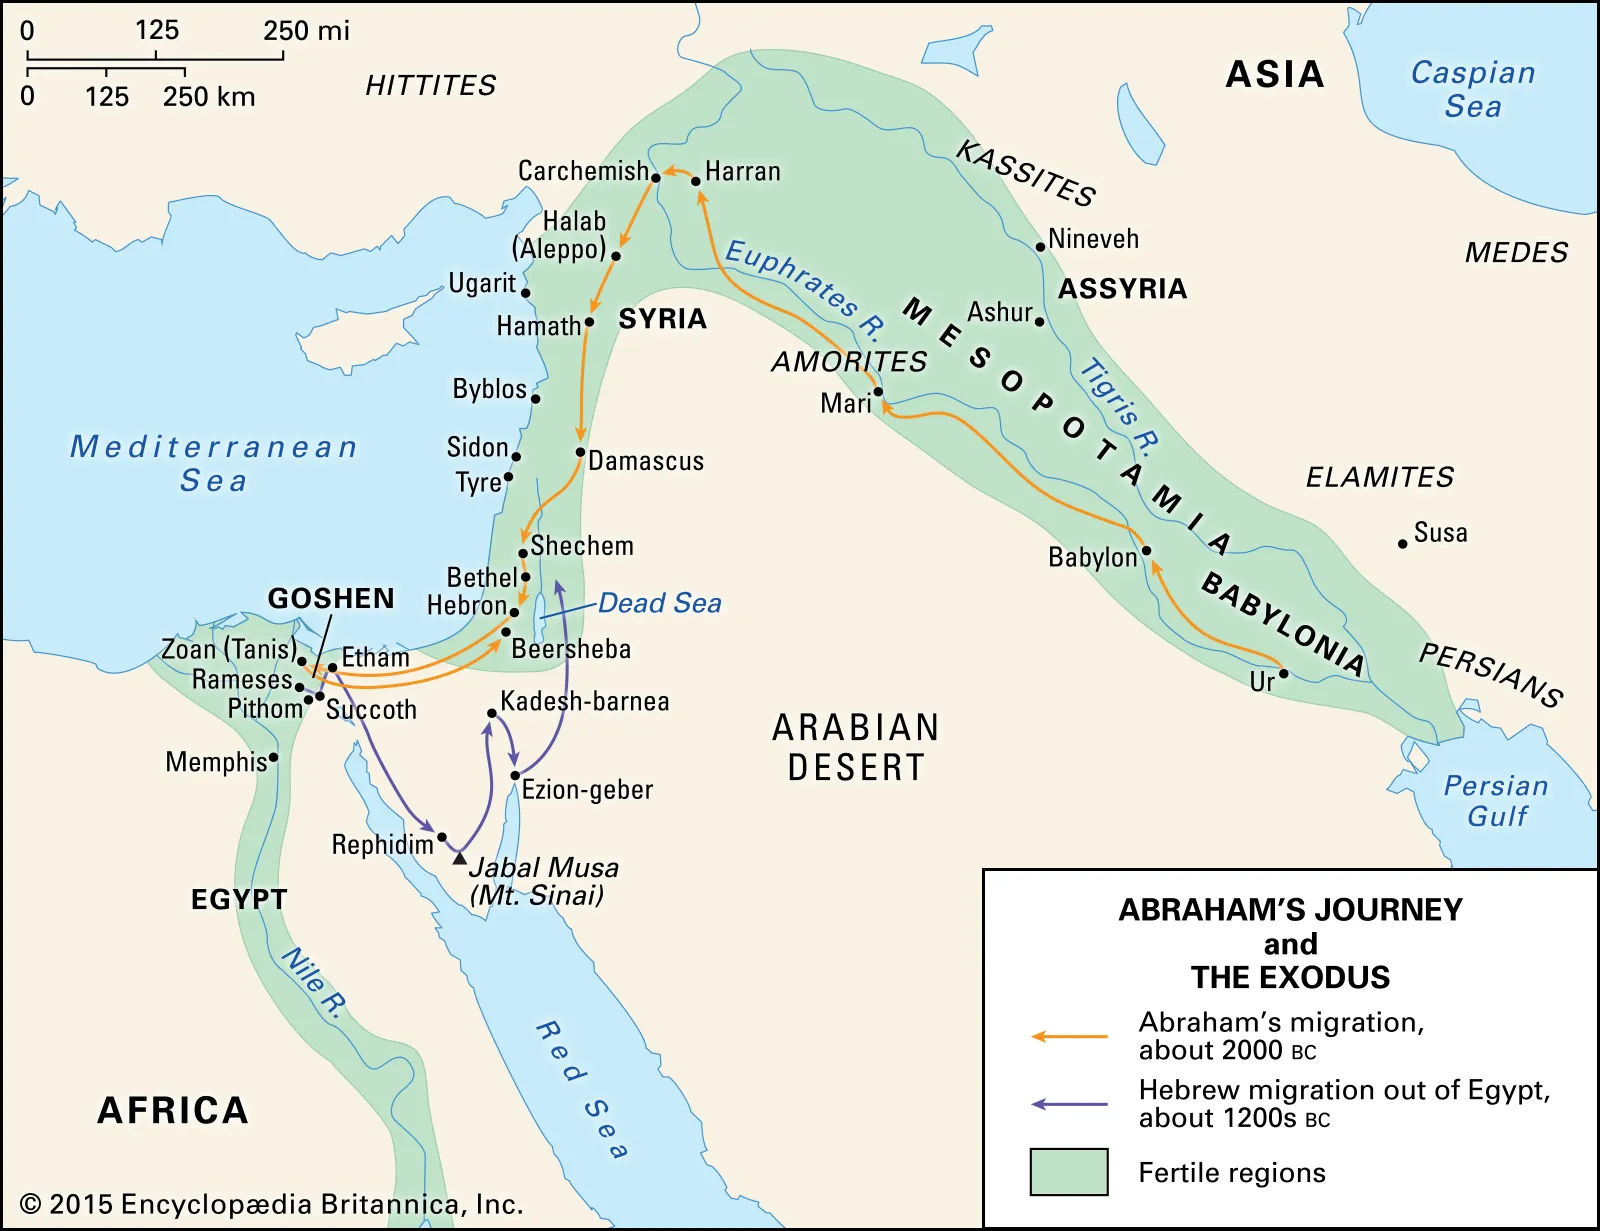
\includegraphics[width=\textwidth]{ZongJie/bibleChildren/fig/abraham}
\end{figure}

\begin{figure}[H]
\centering 
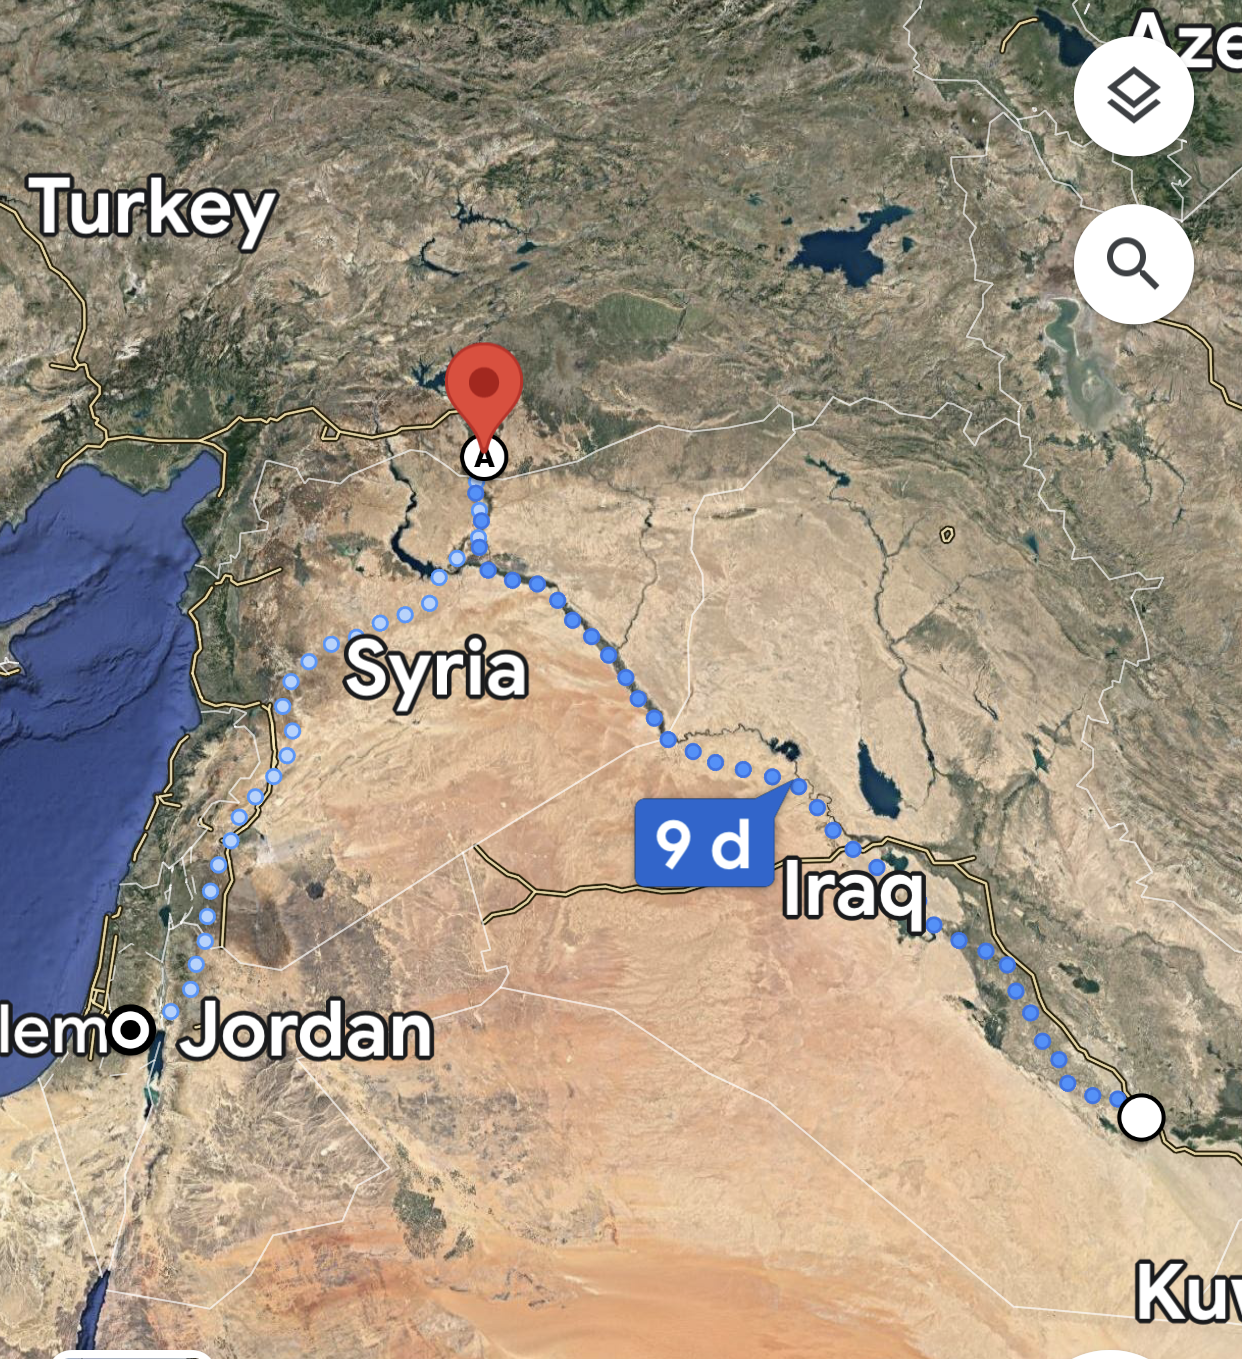
\includegraphics[width=\textwidth]{ZongJie/bibleChildren/fig/Genises}
\end{figure}
\section{questions }
\newpage

\subsection{11:31-33/12:1-7}

\begin{itemize}
\item Find out 
\begin{itemize}
\item 1, What were the promises God gave to Abram? 
\item 2, What was the duty or action that Abram had to do to get God's promises? 
\item 3, What were the blessing or cursess to everyone through Abram?
\end{itemize}
I will make you into a great nation, and I will bless you; I will make your name great, and you will be a blessing. I will bless those who bless you, and whoever curses you I will curse; and all peoples on earth will be blessed through you.”
%\end{itemize}
\item Find out the places of Ur, Harran, Shechem and Bethel from the map.
\item Think about why Abram did not travel from Ur to Shechem, but walk up to Harran, and then down to Shechem?
\end{itemize}

\subsection{15:2-8}
\begin{itemize}
\item What was the concern or worry Abram presented to the God?
\item What were the promises that God gave to Abram? 
%\item In the sentence "and he credited it to him as righteousness", "he" refers to\\
%A, Lord  \hspace{4cm} B, Abram
\item Why the Lord credited Abram as righteousness?
\end{itemize}


\subsection{15:13-21}
\begin{itemize}
\item What would the decendents of Abram do when they become strangers in another country according to God?
\item How long the decendents of Abram dwelt as foreigner in another country?
\item What would the decendents of Abram bring with them when they come out from the foreign country?
\item Why Abram's descendants will not come back to their own country till the 4th generation?
\item Why God would punish that foreign nation?
\end{itemize}

\subsection{17:1-8}
\begin{itemize}
\item Select all the promises that God gave to Abram\\
A. You will become a King;
B. You will be the father of many nations;
C. I will make you a very rich man;\\
D. I will give Canaan as an everlasting possession to you and your descendants;
\item What was the new name of Abram?
\end{itemize}



\subsection{22:1-3}
\begin{itemize}
\item What was the only son's name of Abraham's?
\item Whom did God command Abraham to sacrifice?
\item Why did Abraham cut enough wood before set out for the place God had told him about?
%\item Except of the servants and Isaac, what did Abraham brought with him?
\end{itemize}

\subsection{22:4-8}
\begin{itemize}
\item Abraham told his servants, what he and his son would do?
\item What was the burnt offering in Issac's mind?
\item What was Abraham's answer when Issac asked about the burnt offering?
\item In Abraham's mind, after he had killed his son, Issac would die or not?\\
NIV Hebrew 11:19\\
Abraham reasoned that God could even raise the dead, and so in a manner of speaking he did receive Isaac back from death.
\end{itemize}
\subsection{22:9-18}
\begin{itemize}
\item What burnt offering did God prepared for Abraham to replace his son?
\item What did God know about Abraham after this test?
\item Why did God test Abraham? Didn't God know the result without testing?
\end{itemize}